\documentclass[journal,10pt,onecolumn,draftcls]{IEEEtran}
\usepackage{listings}
\usepackage{wrapfig}
\usepackage{graphicx}
% correct bad hyphenation here
\hyphenation{op-tical net-works semi-conduc-tor}


\begin{document}
%
\title{Individual Project 1: OpenMP}
%

\author{Jeremy Wright}

% The paper headers
\markboth{CSE430 Individual Project 1: OpenMP}
{CSE430 Individual Project 1: OpenMP}

% make the title area
\maketitle


\begin{abstract}
%\boldmath
Parallel code is difficult to write and test, however the OpenMP's set of 
extenstions allow one to add coarse grained parallelism to a system. This paper 
is a look transforming a formerly serial program into a highly parallel one using 
only OpenMP constructs.
\end{abstract}

\IEEEpeerreviewmaketitle

\section{Introduction}

\IEEEPARstart{O}{penMP} allows one to quickly sprinkle bits of parallelism throughout
a serial program and using a profiler such as Intel's Parallel Studio Amplifier, measure 
the speedup.  OpenMP is not a panacea for all parallelism, it only operates over a given 
scope, and you cannot use the parallel for with a C++ iterator.  However despite these 
subtle limitations, OpenMP is an extrememly powerful platform for introducing parallelism
into serial applications and algorithms.

\hfill \today

\section{Game of Life}
Conway's Game of Life is a dramatic illustration that a seemingly complex system
such as cell mitosis can be goverened by a set of fairly simple rules. As a demonstration of
OpenMP's simplicity I implemented a single class implementing the game of life. Then by 
overriding a few key methods, I could dynamically swap out different threading models.

% needed in second column of first page if using \IEEEpubid
%\IEEEpubidadjcol
\subsection{Data Decomposition}
I defined 3 threading models to test OpenMP's performance impact. I defined a threading model
per how I decomposed the data.  I use 3 segmentations division by rows, division by columns, 
division by regions



%
%\begin{figure}[htb]
%\label{fig:inspector_with_debug_symbols}
%\begin{center}
%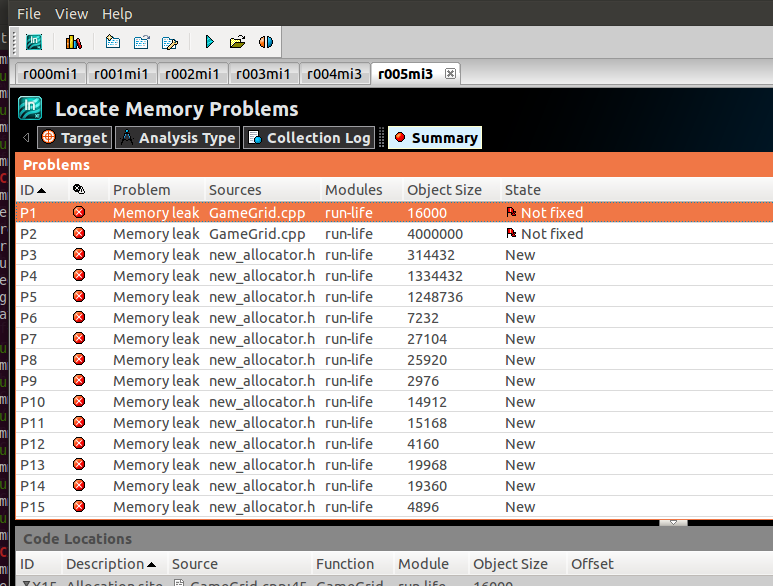
\includegraphics[width=0.5\textwidth]{figures/file8VlHl6_Debug_Symbols.png}
%\caption{Intel Inspector with Debug Symbols enabled.}
%\end{center}
%\end{figure}


\begin{figure}[htb]
\label{fig:inspector_clean_memory}
\begin{center}
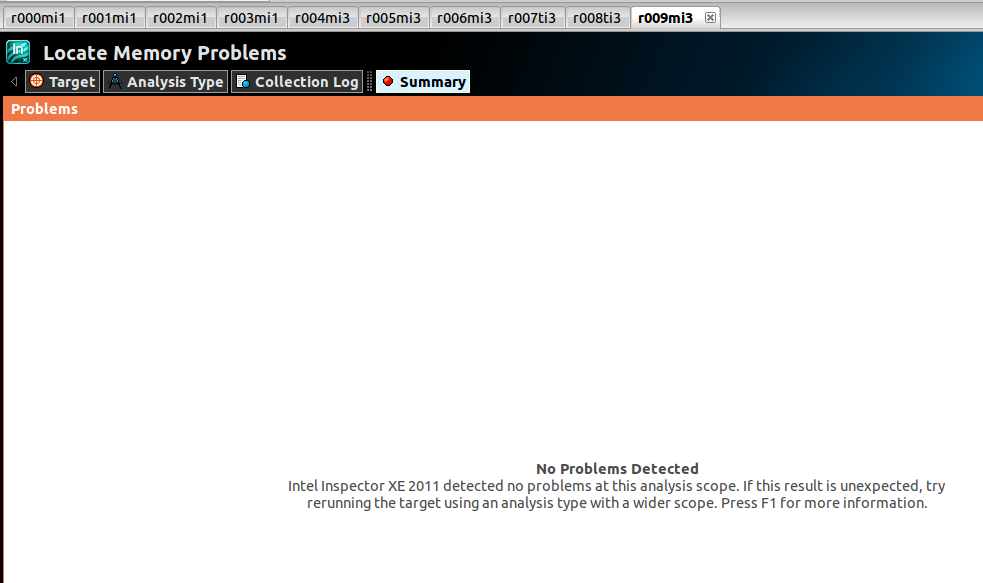
\includegraphics[width=0.5\textwidth]{figures/ChangeSet14_Memory.png}
\caption{Game of Life: All Memory Leaks Fixed.}
\end{center}
\end{figure}

\begin{figure}[htb]
\label{fig:inspector_clean_deadlocks}
\begin{center}
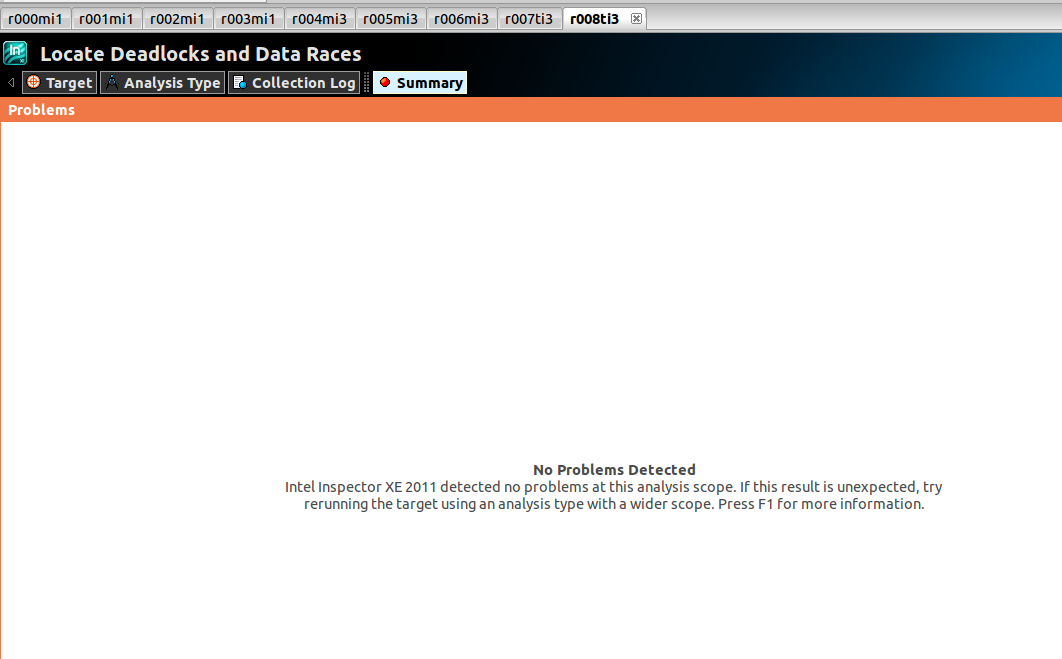
\includegraphics[width=0.5\textwidth]{figures/ChangeSet14.png}
\caption{Game of Life: All Deadlocks and Data Races Fixed.}
\end{center}
\end{figure}

\begin{figure}[htb]
\label{fig:inspector_data_race_allocator}
\begin{center}
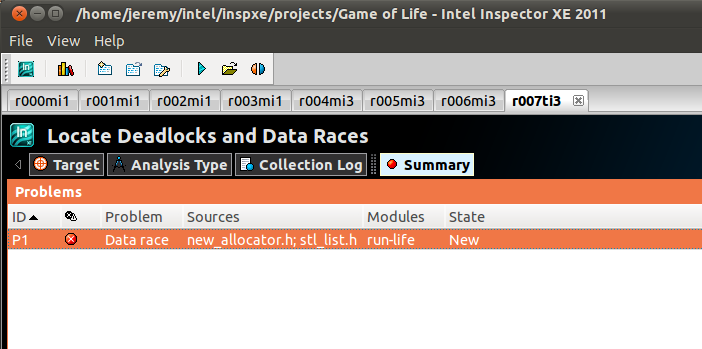
\includegraphics[width=0.5\textwidth]{figures/Data_Race_Anaylsis.png}
\caption{Game of Life: Data Race found on the Update List.}
\end{center}
\end{figure}

\begin{figure}[htb]
\label{fig:matrix_dynamic_schedule_cpu_usage}
\begin{center}
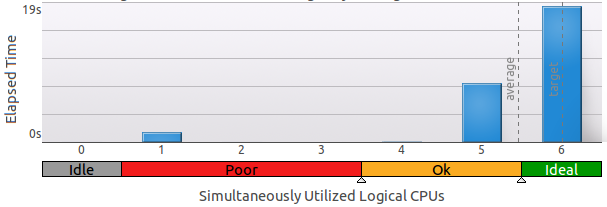
\includegraphics[width=0.8\textwidth]{figures/matrix_dynamic_schedule_cpu_usage.png}
\caption{Matrix Multiply CPU Usage using Dynamic Thread Balancing.}
\end{center}
\end{figure}

\begin{figure}[htb]
\label{fig:matrix_dynamic_schedule_concurrency}
\begin{center}
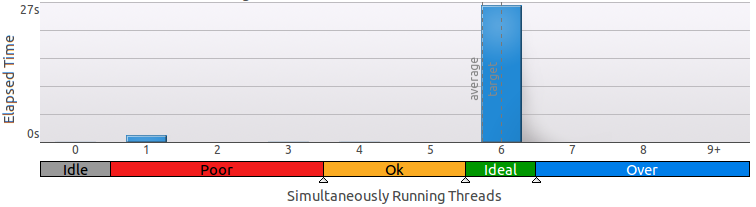
\includegraphics[width=0.8\textwidth]{figures/matrix_dynamic_schedule_thread_concurrency.png}
\caption{Matrix Multiply Thread Concurrency using Dynamic Thread Balancing.}
\end{center}
\end{figure}

\begin{figure}[htb]
\label{fig:matrix_wo_dynamic_schedule_cpu_usage}
\begin{center}
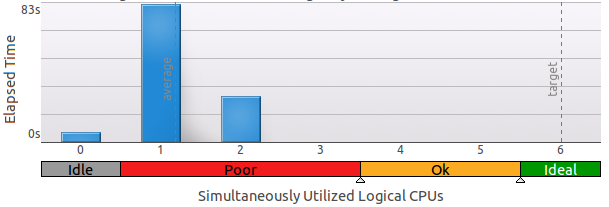
\includegraphics[width=0.8\textwidth]{figures/matrix_without_dynamic_schedule_cpu_usage.png}
\caption{Matrix Multiply CPU Utilization using Standard Parallel for.}
\end{center}
\end{figure}

\begin{figure}[htb]
\label{fig:matrix_wo_dynamic_schedule_concurrency}
\begin{center}
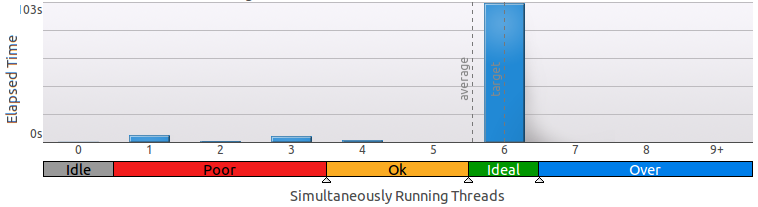
\includegraphics[width=0.9\textwidth]{figures/matrix_without_dynamic_schedule_thread_concurrency.png}
\caption{Matrix Multiply Thread Concurrency using with Standard Parallel for.}
\end{center}
\end{figure}



\begin{figure}[htb]
\label{fig:12_threaded_matrix_cpu_usage}
\begin{center}
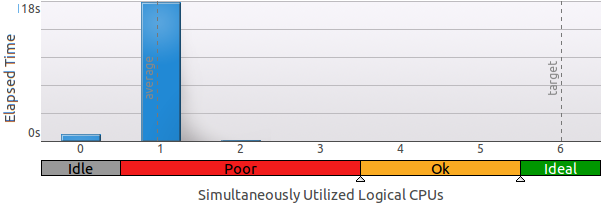
\includegraphics[width=0.8\textwidth]{figures/12_threaded_matrix_thread_cpu_usage_histogram.png}
\caption{CPU Utilization forcing 12 threads.}
\end{center}
\end{figure}

\begin{figure}[htb]
\label{fig:12_threaded_matrix_concurrent}
\begin{center}
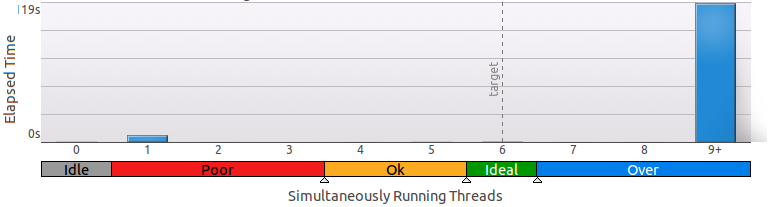
\includegraphics[width=0.8\textwidth]{figures/12_threaded_matrix_thread_concurrent_histogram.png}
\caption{Thread Concurrency forcing 12 threads.}
\end{center}
\end{figure}

\subsection{Intertask Dependency}


\section{Matrix Multiplication}

\subsection{Dynamic Load Balance}

\begin{equation}
\sum\limits_{a}^b (i + 1) = \frac{-(a + b + 2)(a - b -1)}{2}
\end{equation}
a and b define column numbers.  This equation counts the number of 1's in the 
column of an upper triangular matrix. Use this equation one can balance the number of 
multiplications across sets of columns.  For a 2000 column matrix across 6 processors 
we have the following set of equations.
\begin{eqnarray}
\lefteqn{\frac{-(0 + b + 2)(0 - b -1)}{2}} \\
& = & \frac{-(b + c + 2)(b - c -1)}{2} \\
& = & \frac{-(c + d + 2)(c - d -1)}{2} \\
& = & \frac{-(d + e + 2)(d - e -1)}{2} \\
& = & \frac{-(e + 1999 + 2)(e - 1999 -1)}{2}
\end{eqnarray}
One could use Newton's method. This will determine the precise slice of columns which 
will give an even split. This however is non-trivial. This bookkeeping has a diminishing 
return since OpenMP makes this much simplier.

OpenMP has a accepts a number of parameters called clauses. The Scheduling clause allows
for a dynamic load balancing across the OpenMP threads. 

\label{lst:AutomaticLoadBalancing}
\lstset{language=C,
    breaklines=true,
    basicstyle=\footnotesize,
    caption={Automatic Load Balancing with schedule clause},
    captionpos=b}
\begin{lstlisting}
int const chunk = size%omp_get_num_threads();
#pragma omp parallel for schedule(dynamic, chunk)
\end{lstlisting}
Solving this load imbalance is simple as code Listing \ref{lst:AutomaticLoadBalancing}.


\section{Conclusion}
OpenMP makes adding parallelism to a given program easy. The constructs allow one to sprinkle
parallel code throughout the program, and the measure the performance boost. Sometimes it
may be prudent to dive in deeper and manually thread some section of code, but if OpenMP
meets the need, then its a low-cost mechanism, widely supported mechanism.



\appendices
\section{Intel Parallel Studio}
To evaluate the memory tool, I intentionally put some memory leaks in my code 
to see what parallel studio would do.  Valgrind's memory manager finds a lot of 
false positives.You have to wade through piles of innocuous "errors" before you 
find the real ones. Valgrind is excellent, and it does find all the errors but, 
I have found, there is a learning curve on knowing what errors are real, and 
which are superficial. 

It is really satisfying to see the No Memory Leaks found on the Intel tool. I am 
confident that the report is accurate, whereas with Valgrind I'm never 100\% sure that I recovered all my bugs.

For the performance profiling, the profile does slow down execution just as 
Valgrind, but the slowness didn't seem to be as excessive.  The Intel tool 
seemed to profile faster than Valgrind does.  This is purely subjective, as 
I didn't make any comparative measurements.  Some of the graphs are hard to 
understand. And I would really like to sprinkle profile pragma's throughout my 
code to profile smaller sections e.g at the scope level. I don't know of a tool 
that does this (Maybe a thesis topic :-).  But something that allows you to name 
profile sections that the will be reported separately.  

It's great tool suite. I don't have an Intel processor, so some of the profilers 
wouldn't work, and the errors were non-obvious, but overall the tool is great, and 
I really like that it runs on Linux.

\begin{figure}[htb]
\label{fig:intentional_memory_leak}
\begin{center}
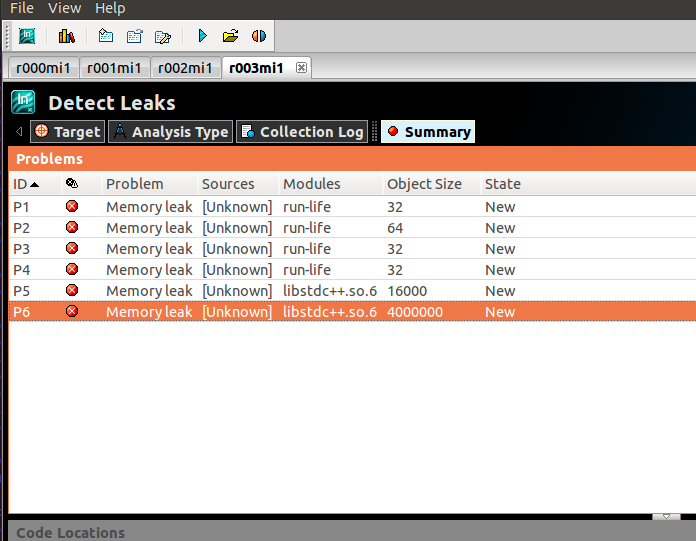
\includegraphics[width=0.8\textwidth]{figures/fileMep7k0_Memory_Analysis.png}
\caption{Intel Inspector with Debug Symbols enabled.}
\end{center}
\end{figure}


\listoffigures

% that's all folks
\end{document}


